
\chapter{Advanced usage: Custom analysis}
\label{custom}

\section{Conveyor}

All offered analysis tools provided by the MGX platform are implemented as workflows
for the Conveyor workflow engine developed by Dr. B. Linke (TODO:cite). Within Conveyor,
tools are provided as so-called ''nodes'', which resemble individual processing steps
and which are used to implement novel analysis methods by simply arranging and connecting
them into a larger workflow. Conveyor currently includes plugins providing typical
bioinformatics tools like BLAST or HMMer, but has recently been extended with dedicated
plugins aimed at metagenome analysis, like MetaCV, MetaPhyler or MetaPhlAn, which all
perform taxonomic analysis.
A dedicated Conveyor plugin provides access to MGX data structures, thereby enabling the
analysis of metagenomes stored in the MGX system with processing tools provided by Conveyor
itself.
While workflow definitions are stored in a XML-based format, a graphical user interface,
the Conveyor designer (\ref{designer}), enables users to implement new analysis by simply
placing and connecting nodes.

\begin{figure}[ht]
\centering
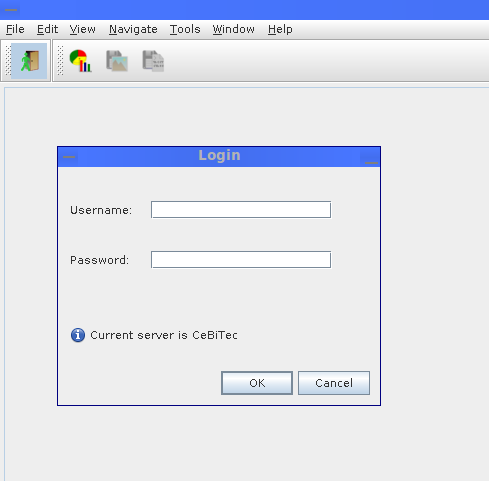
\includegraphics[width=.8\textwidth]{img/login-screen}
\caption['Conveyor Designer]{The Conveyor Designer application allows easy and user-friendly
development of custom analysis algorithms in a graphical way.}
\label{designer}
\end{figure}

As Conveyor is actively developed and new tools are continously integrated, giving a thorough
introduction is beyond the scope of this document. The most up-to-date documentation describing
Conveyor itself and the Conveyor Designer in particular can be found at the Conveyor web
site \url{http://conveyor.CeBiTec.Uni-Bielefeld.DE}

\section{Workflow requirements}

In order to design custom Conveyor workflows for later usage within the MGX platform, there
are several constraints to be met which will be described in more detail.

need MGX node\\
accessing sequences\\
filtering sequences\\
creating attribute types\\
annotating attributes\\
example workflow\\


